\section{Tutorial project}
    The aim of the tutorial project is to provide an easy way to explore the IDE without reading long documents.
    The tutorial project can be opened from the [Main~Menu] -> [Help] -> [Tutorial~Project]. Demonstration project
    should introduce a new user into the basics of usage of this IDE, this generally covers the most common functions
    like assembling the code, running simulator, and so on.
    \begin{figure}[h]
        \centering
        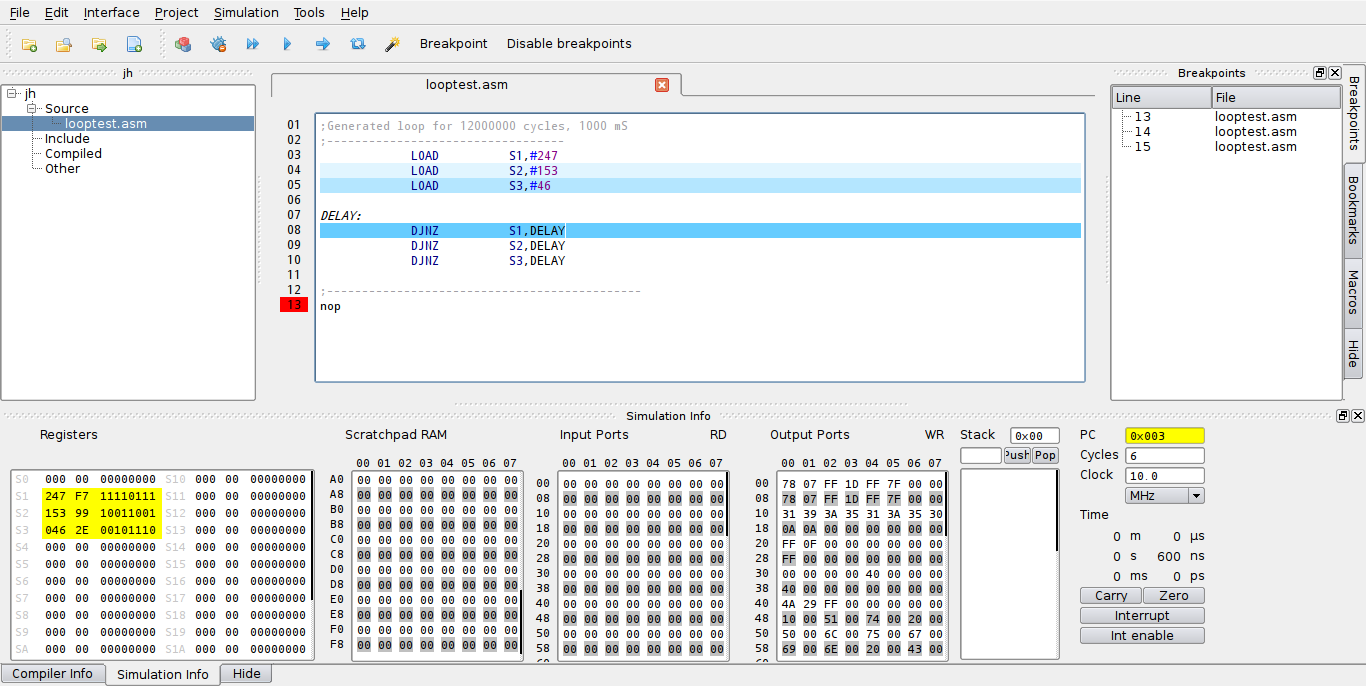
\includegraphics[width=\textwidth]{img/demonstration_1.png}
        \caption{Tutorial project}
    \end{figure}

\section{Your first project}
    (NOTE: We recommend that you to go through the Tutorial Project first.) There is not too much you have to do to start you first project in MDS, to keep things simple:
    \begin{itemize}
        \item Click on [Main~Menu] -> [Project] -> [New~Project].
        \item Choose a name for your project and directory in which you want to store files created in the IDE.
        \item On next tab you can adjust size of the scratch-pad and program memory, or change default interrupt vector.
        \item On Compiler tab you can choose files to generate by the assembler.
        \item Then click OK, and you have your project.
        \item Click on [Main~Menu] -> [File] -> [New~Project~File].
        \item Edit your file as you wish, and save it by clicking on [Main~Menu] -> [File] -> [Save~File].
    \end{itemize}

    \begin{table}[h!]
        \begin{tabular}{ccc}
            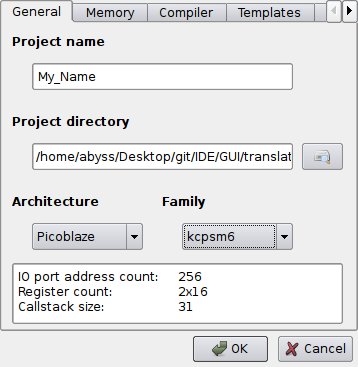
\includegraphics[width=.33\textwidth]{img/project_1.png}
                &
            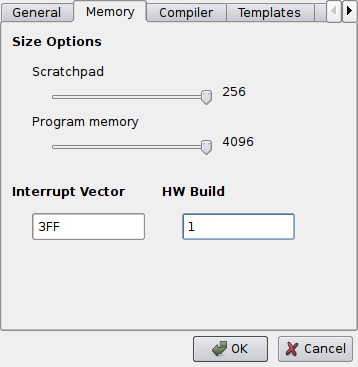
\includegraphics[width=.33\textwidth]{img/project_2.png}
                &
            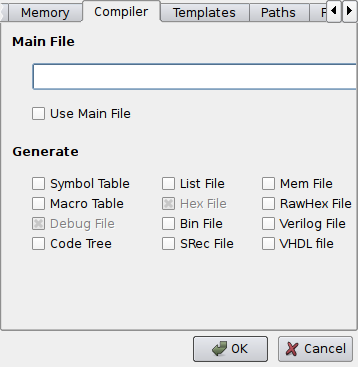
\includegraphics[width=.33\textwidth]{img/project_3.png}
                \\
            General & Memory & Compiler
        \end{tabular}
    \end{table}

    To use what you have just created:
    \begin{itemize}
        \item
            To assemble your file click on [Main~Menu] -> [Project] -> [Compile].
        \item
            To start simulation click on [Main~Menu] -> [Simulation] -> [Start~Simulation].
        \item
            Compiled files suitable for loading into FPGA can be found in the directory which you choose to be your project directory. Types of these files, and therefore their purpose, can be easily determined by their extensions\footnote{These file extensions are only recommended, the actual extensions can be set by user at any time.}:
            \begin{description}
                \item [.rawhex] is HEX file suitable for JTAG loaders,
                \item [.mem] is a decimal representation of the machine code suitable for a number of various tools,
                \item [.vhd] is VHDL code with your machine code (generated from template which can be chosen by user),
                \item [.lst] is code listing,
                \item [.stbl] is table of symbols,
                \item [.mtbl] is table of macros,
                \item [.ihex] is Intel 8 Hex,
                \item [.srec] is Motorola S-Record,
                \item [.bin] is plain binary file,
                \item [.dbg] is a file used the simulator for simulation, it has no other purpose,
                \item [.v] is Verilog code with your machine code (generated from template which can be chosen by user),
                \item [.ctr] is so called code tree, this file has normally no application for regular users, it contains textual representation of raw output from the syntax analyzer.
            \end{description}
    \end{itemize}

\section{Short introduction to MDS macro-assembler}
    This assembler uses almost the same syntax as the Xilinx assembler for PicoBlaze but there are some differences:

    \begin{description}
        \item[Default radix is decimal, not hexadecimal.]~\\
            You can use different radix for each numerical literal, if you do not specify radix, it's decimal by default. For hexadecimal radix use `0x' prefix: 0x1a, 0xbc, 0x23, ...; for octal radix use `0' (zero) prefix: 076, 011, 027, ...; for binary radix use `0b' prefix: 0b11001100, 0b10101010, 0b11111111, ...; for ASCII value put the character in single quotes: 'a', 'A', '3', ... Suffix notation is also supported: 80h (hex.), 128d (dec.), 200q (oct.), 10000000b (bin.), for ASCII characters, you can also use C language escape sequences: \verb"'\0'"~(NUL), \verb"'\n'"~(LF), \verb"'\r"~(CR), \verb"'\t"~(TAB), ...
        \item[Addressing mode specification is mandatory.]~\\
            For immediate addressing use `\#' prefix: \texttt{LOAD~S0,~\#0xAB}; for indirect addressing you ``@'' prefix: ``\texttt{STORE~S0,~@S1}''; for direct addressing use no prefix: ``\texttt{LOAD~S0,~S1~+~3}'' (this loads S0 with S4).
        \item[This assembler is case insensitive.]~\\
            ``\texttt{load~S0,~S1}'' is the same as ``\texttt{LOAD~s0,~s1}'', or ``\texttt{Load~S0,~s1}''.
        \item[This assembler supports user defined macro instructions, and expressions.]~\\
            ``\texttt{LOAD~S0,~\#(2~+~3~*~8)}'', etc. please refer to the Tutorial Project, and the Quick User Guide for brief introduction, or to later pages in this manual for detailed description.
    \end{description}
